\documentclass[a4paper,12pt]{article}
\usepackage[left=1.5cm, right=1.5cm, top=2cm,bottom=2cm]{geometry}
\usepackage{amsmath, amssymb, amsfonts, amsthm}
\usepackage{multicol}
\usepackage{enumerate}
\usepackage{pgfplots}
\usepackage{tikz}

% https://tex.stackexchange.com/questions/29834/closed-square-root-symbol
\usepackage{letltxmacro}
\makeatletter
\let\oldr@@t\r@@t
\def\r@@t#1#2{%
\setbox0=\hbox{$\oldr@@t#1{#2\,}$}\dimen0=\ht0
\advance\dimen0-0.2\ht0
\setbox2=\hbox{\vrule height\ht0 depth -\dimen0}%
{\box0\lower0.4pt\box2}}
\LetLtxMacro{\oldsqrt}{\sqrt}
\renewcommand*{\sqrt}[2][\ ]{\oldsqrt[#1]{#2}}
\makeatother

\newcommand{\novografico}[3]{
\begin{tikzpicture}
    \begin{axis}[
        grid=both,
        grid style={line width=.1pt, draw=gray!50, dashed},
        major grid style={line width=.2pt,draw=gray!50, dashed},
        axis lines=middle,
        enlargelimits,
        samples=75,
        domain=#1,
        width=5cm,
        height=5cm,
        xlabel=$x$,
        ylabel={$#3$},
        xlabel style={at={(current axis.right of origin)}, anchor=west},
        ylabel style={at={(current axis.above origin)}, anchor=south},
        unbounded coords=jump
    ]
    \addplot[blue, thick] {#2}; 
    \end{axis}
\end{tikzpicture}
}

\begin{document} 
  
\section*{Piape Matemática} 
\textbf{Módulo IV - Tudo é função}\\
\textbf{Exercícios Aula 05}    

\begin{multicols}{2} 
 
\paragraph*{1.} Identifique cada tipo de função conforme o gráfico: 
\begin{itemize}
    \item Função polinomial
    \item Função exponencial
    \item Função logarítmica
    \item Função constante
    \item Função afim
    \item Função racional
    \item Função trigonométrica
\end{itemize}

\novografico{-4:2}{x^2 + 3*x}{f(x)}
\novografico{-2:2}{x^3 - 2*x}{g(x)}    

\novografico{0.1:3}{ln(x)}{h(x)}
\novografico{-2:2}{exp(x)}{i(x)}

\novografico{-3:3}{2-x}{j(x)}
\novografico{-2:2}{1}{l(x)}

\novografico{-3:7}{sin(deg(x))}{m(x)}
\novografico{-1.5:1.5}{tan(deg(x))}{n(x)}

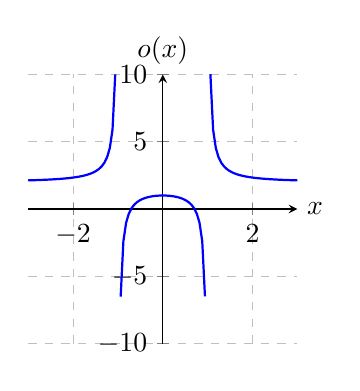
\begin{tikzpicture}
    \begin{axis}[
        grid=both,
        grid style={line width=.1pt, draw=gray!50, dashed},
        major grid style={line width=.2pt,draw=gray!50, dashed},
        axis lines=middle,
        samples=100,
        domain=-3:3,
        width=5cm,
        height=5cm,
        xlabel=$x$,
        ylabel={$o(x)$},
        xlabel style={at={(current axis.right of origin)}, anchor=west},
        ylabel style={at={(current axis.above origin)}, anchor=south},  
        unbounded coords=jump,
        ymax=10,
        ymin=-10
    ]
    \addplot[blue, thick, y filter/.expression={abs(y)>20? inf: y}] {2+1/(x^2-1)}; 
    \end{axis}
\end{tikzpicture}
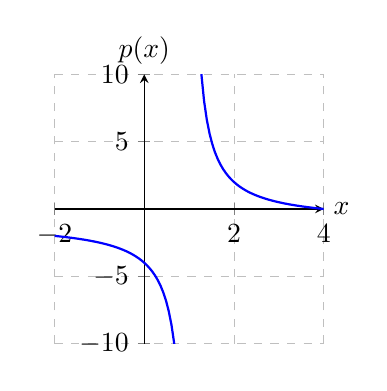
\begin{tikzpicture}
    \begin{axis}[
        grid=both,
        grid style={line width=.1pt, draw=gray!50, dashed},
        major grid style={line width=.2pt,draw=gray!50, dashed},
        axis lines=middle,
        samples=100,
        domain=-2:4,
        width=5cm,
        height=5cm,
        xlabel=$x$,
        ylabel={$p(x)$},
        xlabel style={at={(current axis.right of origin)}, anchor=west},
        ylabel style={at={(current axis.above origin)}, anchor=south},  
        unbounded coords=jump,
        ymax=10,
        ymin=-10
    ]
    \addplot[blue, thick, y filter/.expression={abs(y)>20? inf: y}] {-1+3/(x-1)}; 
    \end{axis}
\end{tikzpicture}

\end{multicols}

\vspace*{\fill}
{\footnotesize
\paragraph*{Gabarito} \hspace*{\fill}\\
\textbf{1.}   
$f(x)$ é uma função polinomial de grau 2;
$g(x)$ é uma função polinomial de grau 3;
$h(x)$ é uma função logarítmica;
$i(x)$ é uma função exponencial;
$j(x)$ é uma função afim;
$l(x)$ é uma função constante;
$m(x)$ é uma função trigonométrica;
$n(x)$ é uma função trigonométrica;
$o(x)$ é uma função racional;
$p(x)$ é uma função racional.
}
\end{document}